\documentclass[11pt]{report} %size of font and type of layout
\usepackage[a4paper,margin=1in]{geometry}

\usepackage{pgfplots}
\usepackage{tikz}
\usepackage{xfrac}
\usepackage[super]{nth} %allow 1st, 2nd by typing \nth{1}, \nth{2}
\usepackage[title,titletoc,page]{appendix} %for using appendices
\usepackage{graphicx} %have images
\usepackage{chngcntr} %be able to make figures go 1, 2, 3 instead of 1.1, 1.2, 1.3, etc
\usepackage{subcaption} %have subfigures
\usepackage{wrapfig} %be able to wrap text around figures
\usepackage{amsmath} %a way to typeset maths
\usepackage{amssymb} %able to type maths symbols
\usepackage{textcomp} %so we can use \textdegree to get degree symbol
\usepackage[parfill]{parskip} %remove paragraph indentation
\usepackage{setspace} %be able to set line spacing
\usepackage{tocloft} %more control over table of contents, list of figures, etc
\usepackage{ltxtable} %get tabularx split over pages
\usepackage[english]{babel} %english-specific charaters and language rules
\usepackage{url} %type urls
\usepackage{parskip} %space between paragraphs
\usepackage[UKenglish]{isodate} %change date format
%\usepackage[hang,flushmargin]{footmisc} %no indents in footers
%\usepackage{verbatimbox} %able to use addvbuffer to change spaces before and after tables
\usepackage{pdfpages} %insert PDF pages
%\usepackage{titletoc} %create a small table of contents at the start of each section
\usepackage{microtype} %improves spacing between words and letters
\usepackage[nodayofweek]{datetime} %use \today to get the date
\usepackage[inline]{enumitem} %have inline lists
\usepackage{fancyhdr}		%for getting customized headers
\usepackage{lastpage}		%enable getting the total of the pages
%\usepackage{floatrow} %use for indicating figures' sources
%\usepackage{showframe} %show margins on page
\usepackage[hidelinks]{hyperref} %hyperlinks in pdf
\usepackage{cleveref} %automatic referencing
\usepackage{bookmark}
\DeclareGraphicsExtensions{.pdf,.png,.jpg,.eps} %can just give images' names
\usepackage{epstopdf} %allows for encapsulated postscript vector images, better quality and scalable
\usepackage[none]{hyphenat}		%kills all word breaks that were in annoying places

%--------------------------heading spacings----------------------------%
\usepackage{titlesec} %be able to change title settings
	\titleformat{\chapter}{\normalfont\huge\bfseries}{\thechapter.}{1em}{} %have number before chapter title
	\titlespacing{\chapter}{0pc}{0pc}{0pc} %have nice spacing after chapter title {indent} {before} {after}
	\titlespacing{\section}{0pc}{1pc}{0pc} %have nice spacing after section title {indent} {before} {after}
	\titlespacing{\subsection}{1pc}{1pc}{0pc} %have nice spacing after subsection title {indent} {before} {after}
	\titlespacing{\subsubsection}{0pc}{0pc}{-1pc} %have nice spacing after subsection title {indent} {before} {after}
	\titlelabel{\thetitle.\quad} %full stop after the number in the heading title
\usepackage{etoolbox} %remove page break before chapter heading
	\makeatletter
	\patchcmd{\chapter}{\thispagestyle{plain}}{\thispagestyle{fancy}}{}{} %allows the header/footer on chapter pages
	\patchcmd{\chapter}{\if@openright\cleardoublepage\else\clearpage\fi}{}{}{}
	\makeatother
%----------------------------figures & lof (list of figures)-----------------------------%
\renewcommand{\cftfigfont}{Figure } %list of figures includes "Figure"
\newcommand*{\noaddvspace}{\renewcommand*{\addvspace}[1]{}}\addtocontents{lof}{\protect\noaddvspace} %equal line spacing in the list of figures
\setlength{\cftfigindent}{0pt} %remove indentation from figures in lof
\usepackage{float} %able to use H to force figures to go here
%\floatstyle{boxed}	%this will place a thin border around my figures
%\restylefloat{figure}
\AtBeginEnvironment{figure}{\vspace{10pt}} %spacing before figure
\AtEndEnvironment{figure}{\vspace{-10pt}} %spacing after figure
\setlength{\abovecaptionskip}{10pt} %spacing before figure caption
\setlength{\belowcaptionskip}{5pt} %spacing after figure caption
\usepackage[justification=centering,font={normalsize, it}]{caption} %control caption text
%----------------------------tables & lot------------------------------%
\renewcommand{\cfttabfont}{Table } %list of tables includes "Table"
\setlength{\cfttabindent}{0pt} %remove indentation from tables in lot
\usepackage{tabularx} %word wrap in tables
\usepackage{longtable} %allow tables to go over multiple pages
\usepackage{multirow} %make cells span multiple rows in tables
\captionsetup{belowskip=5pt,aboveskip=4pt}
\newcolumntype{L}{>{\centering\arraybackslash}m{3cm}} %centre and wrap text in tables
\usepackage{booktabs} %use \toprule, \midrule, \bottomrule and \cmidrule for better spacing in tables
\usepackage{pbox} %force line break in a table cell
%---------------------------create own lists---------------------------%
\newlistof{example}{exp}{List of Examples} %create own lists
\newcommand{\example}[1]{ %create own lists
	\refstepcounter{example} %create own lists
	\par\noindent\textbf{Example \theexample. #1} %create own lists
	\addcontentsline{exp}{example} %create own lists
	{\protect\numberline{\thechapter.\theexample}#1}\par} %create own lists
%---------------------------------font---------------------------------%
%\sfdefault = calibri-like font, \rmdefault = times new roman-like
\renewcommand\UrlFont{\rmfamily}
\renewcommand{\familydefault}{\rmdefault}
%----------------------------------------------------------------------%
\begin{document}
\begin{onehalfspace} %single line spacing
%\counterwithout{figure}{chapter} %makes figures go 1, 2, 3 instead of 1.1, 1.2, 1.3, etc
%\counterwithout{table}{chapter} %makes tables go 1, 2, 3 instead of 1.1, 1.2, 1.3, etc
%\counterwithout{section}{chapter} %make sections 1, 2, 3 not 1.1 etc
\pretolerance=10000 %disable hyphenating at line breaks
\abovedisplayskip=5pt %remove space before equations
\belowdisplayskip=5pt %remove space after equations
\cleanlookdateon %remove current date format to replace with [UKenglish]{isodate}
%\let\savenumberline\numberline\def\numberline#1{\savenumberline{#1.}} %adds dot after chapter title in toc, comment this out to get appendices to work and not cause spacing errors.
\AtEndEnvironment{itemize}{\vspace{-5pt}} %spacing after lists 

\newcommand{\thetitle}	{Business Plan}
\newcommand{\theauthor}	{Roberto Aldera - ALDROB001 \\ Gareth Callanan - CLLGAR010 \\ Luke Goemans - GMNLUK001 \\ Benjamin Scholtz - SCHBEN011 \\ Munawwar Tayob - TYBMUN001 }
\newcommand{\studentnum}{}
\newcommand{\thedate}	{\today}
\newcommand{\coursecode}{EEE4051F}
\newcommand{\coursename}{New Venture Planning}
\newcommand{\staffmember}{Dr. Peter Martinez}

\pagenumbering{gobble}	%no page number for title page
\renewcommand\headrulewidth{0pt}	%get rid of stray header underline
	\begin{center}
\begin{minipage}{1\textwidth}
\begin{center}
	
\begin{center}
\includegraphics[width=1\linewidth]{"UCThoriz"}
\end{center}
\vskip20pt
\Large{Faculty of Engineering and the Built Environment}\\
Department of Electrical Engineering\\
\coursecode
\vskip10pt
\begin{figure}[H]
\centering
\hspace{-3em}
\includegraphics[width=0.6\textwidth]{images/uvuka_logo_ben}
\vskip20pt
\end{figure}
\hrule
\vskip20pt
\Huge\sc{\thetitle}
\vskip20pt
\hrule
\vskip20pt
\Large\textnormal{\textbf{Team 5:}\\
\theauthor\\
\vskip10pt
\textbf{Lecturer:} \staffmember
\vskip20pt
\hrule
\vskip20pt
\thedate\\}
%\textbf{\assignmentname}
\end{center}
\end{minipage}
\end{center}

\newpage 	
%	\chapter*{Plagiarism Declaration}
We know that plagiarism is wrong. Plagiarism is to use another's work and pretend that it is our own.

We have used the IEEE convention for citation and referencing. In this report, all contributions to, and quotations from, the work(s) of other people have been cited and referenced. 

This report is our own work. We have not allowed, and will not allow, anyone to copy our work.
\vskip100pt
\begin{center}
	Signed: \line(1,0){200}
	\vskip20pt
	Dated: \line(1,0){200}
\end{center}

\newpage
	\renewcommand{\contentsname}{Table of Contents} %change table of contents's name from 'contents' to 'table of contents'
\newpage %page break
\phantomsection %for some reason this gets the bookmarks to work

\tableofcontents



%\addcontentsline{toc}{chapter}{Section:} %add "table of contents" to the table of contents
\newpage %page break
\renewcommand\headrulewidth{0.4pt}
\pagenumbering{arabic}	%start the page numbering (and reset it to zero)

\pagestyle{fancy}
\fancyhf{}
\rhead{Group 5}
\lhead{\coursecode \\ \coursename}
\cfoot{Page \thepage \ of \pageref{LastPage}}

%\chapter*{Executive Summary}
%\addcontentsline{toc}{chapter}{Executive Summary}

\newpage
\chapter{Introduction}
This is pretty cool. \\
I want to try add an image...



\begin{figure}[H]
\centering
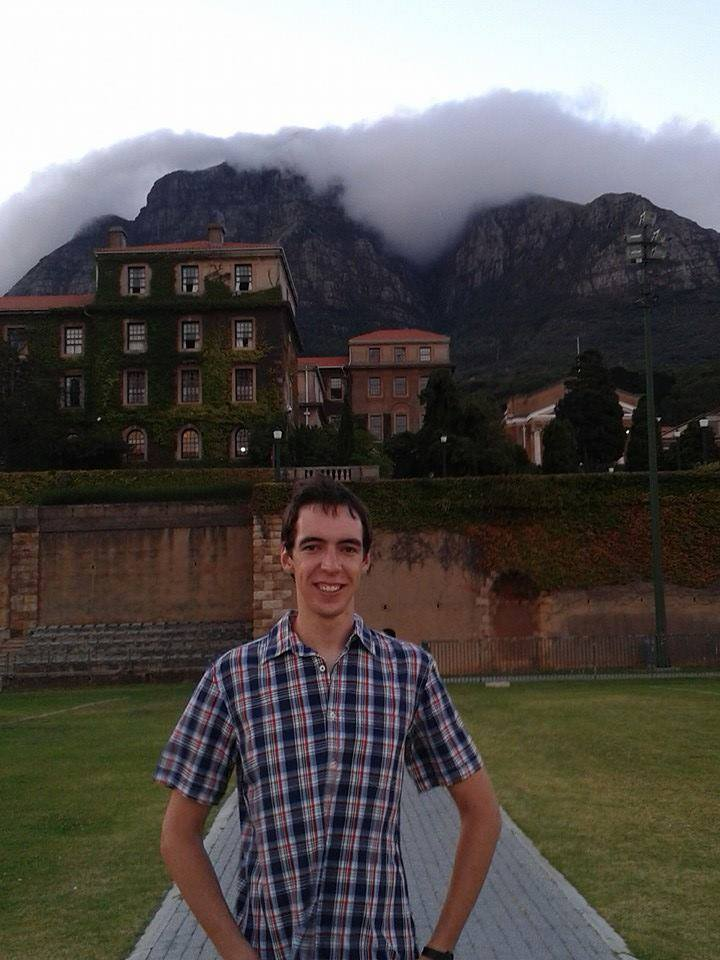
\includegraphics[scale=0.4]{images/garrels}
\caption{Gareth for president!}
\end{figure}



\newpage
\chapter{Product Description}

\newpage
\chapter{Marketing Plan}

%\begin{appendices}
\appendix
\chapter{Insert Here}
\label{app:Insert Here}	
\newpage

\chapter{Another}
\label{app:Another}
\end{appendices}	%for use with appendices
%\newpage
%\bibliography{Aldera_bibliography}
%\bibliographystyle{ieeetran}
%\addcontentsline{toc}{chapter}{Bibliography}

\newpage	%this keeps the header/footer working on the last page. Do not type anything after this.

\end{onehalfspace}
\end{document}

%-------------------------------Figures--------------------------------%
\begin{figure}[H]
\centering
\includegraphics[width=0.4\textwidth]{images/%}
\vskip10pt
\caption[The caption that appears in the list of figures]{The caption that appears under the figure}
\label{fig:exam}
\end{figure}

\begin{figure}[H]
\centering
\begin{subfigure}[t]{0.49\textwidth}
\centering
\includegraphics[width=0.9\linewidth]{images/%}
\caption{This is figure a}
\label{fig:figureA}
\end{subfigure}
\begin{subfigure}[t]{0.49\textwidth}
\centering
\includegraphics[width=0.9\linewidth]{images/%}
\caption{This is figure b}
\label{fig:figureB}
\end{subfigure}
\caption{Caption}
\end{figure}

\begin{wrapfigure}{r}{0.5\textwidth}
\begin{center}
\includegraphics[width=0.48\textwidth]{images/ %}
\end{center}
\caption{A gull}
\end{wrapfigure}

As can be seen in \cref{fig:exam}\\
%-------------------------------Headings-------------------------------%
\chapter{Chapter Title}
\label{ch:Chapter Title}

\section{Section Title}
\label{sec:Section Title}

\subsection{Subsection Title}
\label{subsec:Subsection Title}

\subsubsection{Subsubsection Title}
\label{bb:Subsubsection Title}
%---------------------------Tables and Lists---------------------------%
\renewcommand{\contentsname}{Table of Contents} %change table of contents's name from 'contents' to 'table of contents'
\newpage %page break
\phantomsection %for some reason this gets the bookmarks to work

\tableofcontents



%\addcontentsline{toc}{chapter}{Section:} %add "table of contents" to the table of contents
\newpage %page break
\input{\filepath /list_of_figures.tex}
\input{\filepath /list_of_tables.tex}
\input{\filepath /list_of_example.tex}

\startcontents[chapters] %mini table of contents
\printcontents[chapters]{}{1}{}
\newpage
%-----------------------------Insert Pages-----------------------------%
\includepdf[pages={1}]{ %filename.pdf}
%-------------------------------Appendix-------------------------------%
\startcontents[section]
\printcontents[section]{}{1}{}
\newpage
\addcontentsline{toc}{section}{1. %}
%--------------------------------Citing--------------------------------%
\footnote{\cite{aa}}
\cite{aa,bb}
%--------------------------Custom Bibliography-------------------------%
makebst
%----------------------------Maths & Symbols---------------------------%
http://www.artofproblemsolving.com/Wiki/index.php/LaTeX:Symbols
http://www.tex.ac.uk/tex-archive/info/symbols/comprehensive/symbols-a4.pdf
$Hardcore \: maths \: here \: \therefore \ddot{\theta}^{2} = \left(\dfrac{\omega_{n}}{17a}\right) \times 9$
$$ More \: maths: \sqrt{52} + F_{1} = 6 \times 10^{5} \: Hz$$
$\mathrm{\today}$ %maths in normal font
%---------------------------Lines and Spacing--------------------------%
\noindent\makebox[\linewidth]{\rule{\textwidth}{0.4pt}}
\vspace{11pt}
\hspace{-11pt}
\hphantom{11pt}
%----------------------------Page Numbering----------------------------%
\pagenumbering{gobble} %remove page numbering
\pagenumbering{roman} %roman letters page numbering
\pagenumbering{arabic} %arabic letters page numbering
\setcounter{page}{1} %reset page numbers
%--------------------------------Tables--------------------------------%
\begin{table}[H]
\caption{Caption of table}
\addvbuffer[12pt 8pt]{
\begin{tabularx}{0.3\textwidth}{@{}rcl@{}}
\hline
\multicolumn{3}{@{}c@{}}{\textbf{Title}}\\
\hline
Info	& 3	& mm\\
Item	& 5	& x $\approx$ 34\\
\cline{2-2}
Width	& 4	& miles\\
Depth	& 7	& \pbox{20cm}{This is the first \\ cell}\\
\hline
\label{tab:capt}
\end{tabularx}
}
\end{table}

\begin{tabularx}{\textwidth}{@{}lX@{}}
 & \\
\end{tabularx}

\\
\\
\begin{tabular}{ l l }
 & \\
\end{tabular}
%--------------------------------Lists---------------------------------%
http://en.wikibooks.org/wiki/LaTeX/List_Structures

%TC:ignore
\begin{itemize} \itemsep1pt \parskip0pt \parsep0pt \vspace{-6pt}
%TC:endignore
\item[-] The first item
\item[-] The second item
\item[-] The third etc \ldots
\end{itemize}

\begin{enumerate} [label=\bfseries Exercise \arabic*:]
\item The first item
\item The second item
\item The third etc \ldots
\end{enumerate}

\begin{description}
\item[First] The first item
\item[Second] The second item
\item[Third] The third etc \ldots
\end{description}

\begin{description}
\item[First] \hfill \\
The first item
\item[Second] \hfill \\
The second item
\item[Third] \hfill \\
The third etc \ldots
\end{description}

Inline lists are \begin{enumerate*}[label=\itshape\alph*\upshape)]
\item formatted within their paragraph;
\item usually labelled with letters; and
\item usually have the final item prefixed with
`and' or `or',
\end{enumerate*} like this example.

\example{Your first example}
\label{1st_ex}
\example{Your second example}
\label{2nd_ex}
\example{Your third example. (See example \ref{1st_ex} and \ref{2nd_ex})}
%----------------------------------------------------------------------%
\fi